% Conceptual control groups, not a second rendering of the module UI.
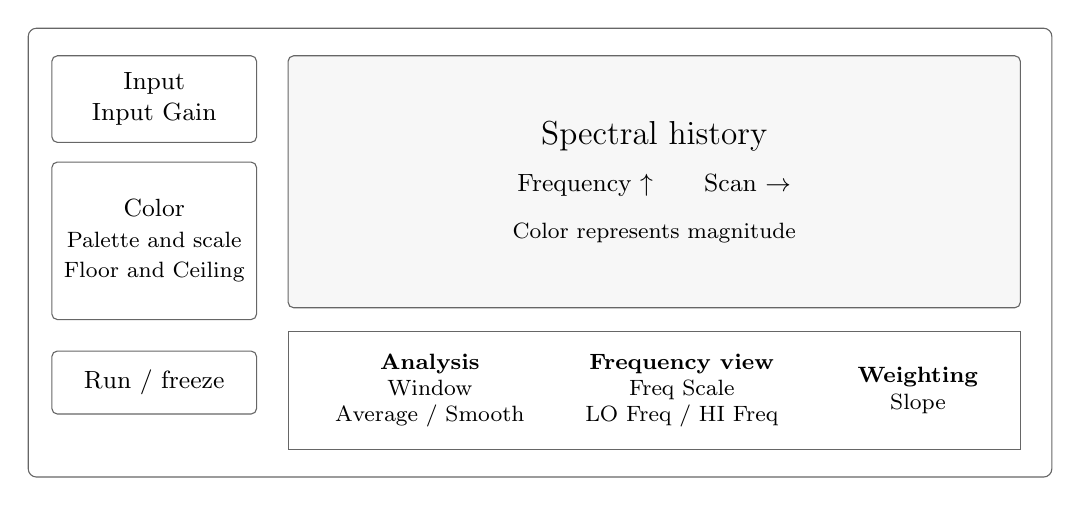
\begin{tikzpicture}[x=1cm,y=1cm,font=\small,
    region/.style={draw=black!60,rounded corners=2pt,align=center},
    label/.style={font=\footnotesize,align=center}]
  \draw[black!60,rounded corners=3pt] (0,0) rectangle (13,5.7);
  \node[region,minimum width=2.6cm,minimum height=1.1cm] at (1.6,4.8)
    {Input\\Input Gain};
  \node[region,minimum width=2.6cm,minimum height=2cm] at (1.6,3)
    {Color\\\footnotesize Palette and scale\\\footnotesize Floor and Ceiling};
  \node[region,minimum width=2.6cm,minimum height=.8cm] at (1.6,1.2)
    {Run / freeze};
  \node[region,fill=black!3,minimum width=9.3cm,minimum height=3.2cm]
    at (7.95,3.75) {\large Spectral history\\[6pt]
      Frequency $\uparrow$\qquad Scan $\rightarrow$\\[6pt]
      \footnotesize Color represents magnitude};
  \draw[black!60] (3.3,.35) rectangle (12.6,1.85);
  \node[label] at (5.1,1.1) {\textbf{Analysis}\\Window\\Average / Smooth};
  \node[label] at (8.3,1.1) {\textbf{Frequency view}\\Freq Scale\\LO Freq / HI Freq};
  \node[label] at (11.3,1.1) {\textbf{Weighting}\\Slope};
\end{tikzpicture}
